\documentclass[border=10pt]{standalone}
\usepackage{tikz}

\tikzstyle{vertex}=[circle,draw,fill=black!20,minimum size=0.6cm,inner sep=0pt]
\tikzstyle{selected vertex} = [vertex, fill=blue!50]
\tikzstyle{edge} = [draw,thick,->]
\tikzstyle{weight} = [font=\small]
\tikzstyle{selected edge} = [draw,line width=3pt,-,red!50, opacity=0.5]
\tikzstyle{ignored edge} = [draw,line width=5pt,-,black!20]

\begin{document}
\noindent
    \centering
    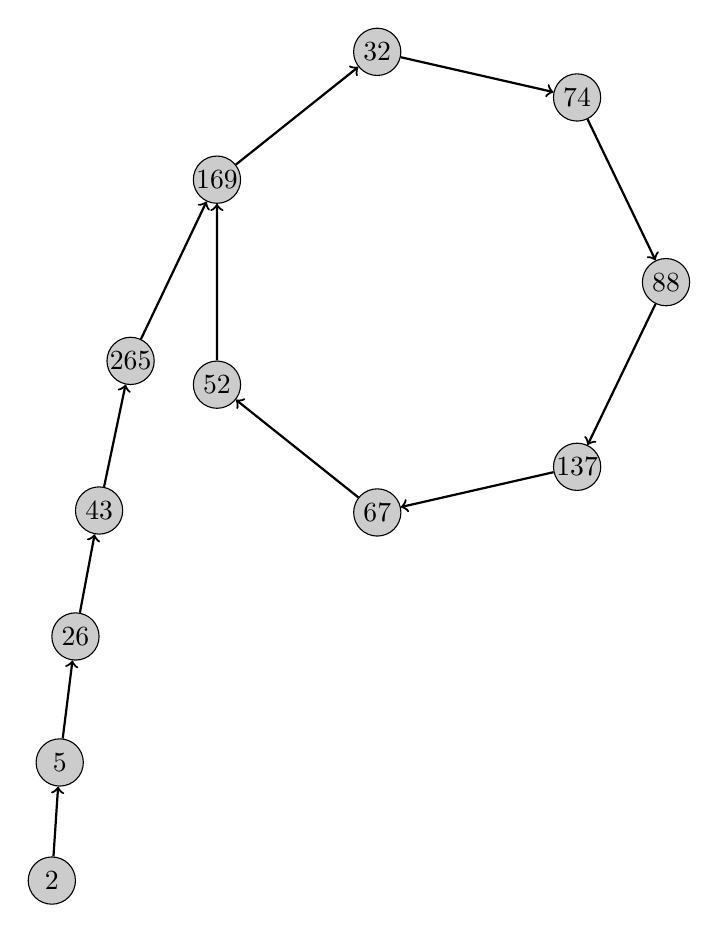
\begin{tikzpicture}[scale=1.0,transform shape,auto,swap]
        \node[vertex] (0) at (3.0, 0.0) {88};
        \node[vertex] (1) at (1.870397, 2.345552) {74};
        \node[vertex] (2) at (-0.667742, 2.924743) {32};
        \node[vertex] (3) at (-2.703026, 1.301403) {169};
        \node[vertex] (4) at (-2.702747, -1.301983) {52};
        \node[vertex] (5) at (-0.667114, -2.924886) {67};
        \node[vertex] (6) at (1.870901, -2.34515) {137};
        \node[vertex] (7) at (-3.8, -1) {265};
        \node[vertex] (8) at (-4.2, -2.9) {43};
        \node[vertex] (9) at (-4.5, -4.5) {26};
        \node[vertex] (10) at (-4.7, -6.1) {5};
        \node[vertex] (11) at (-4.8, -7.6) {2};
        \path[edge] (2) -- node[weight] {} (1);
        \path[edge] (1) -- node[weight] {} (0);
        \path[edge] (0) -- node[weight] {} (6);
        \path[edge] (6) -- node[weight] {} (5);
        \path[edge] (5) -- node[weight] {} (4);
        \path[edge] (4) -- node[weight] {} (3);
        \path[edge] (3) -- node[weight] {} (2);
        \path[edge] (7) -- node[weight] {} (3);
        \path[edge] (8) -- node[weight] {} (7);
        \path[edge] (9) -- node[weight] {} (8);
        \path[edge] (10) -- node[weight] {} (9);
        \path[edge] (11) -- node[weight] {} (10);
    \end{tikzpicture}
\end{document}
